\documentclass{beamer}
\mode<presentation>{\usetheme{Custom}}

\usepackage[orientation=landscape,size=a0,scale=1.4,debug]{beamerposter}
\usepackage[french,english]{babel}
\usepackage[utf8]{inputenc}
\usepackage{graphicx}
\usepackage{xcolor}
\usepackage{tcolorbox}
\usepackage{tikz}


\tikzset{every picture/.style={execute at begin picture={
   \shorthandoff{:;!?};}
}}

\tikzset{rndblock/.style={rounded corners,rectangle,draw,outer sep=0pt}}
\newcommand{\tframed}[2][]{\tikz[baseline=0.1pt]\vspace{0.1cm}\node[rndblock,minimum height=1.5em,#1] (m) {#2} ;}
\newcommand{\hilight}[1]{\textbf{\tframed[blue,fill=blue!10]{#1}}}
\newcommand{\whilight}[1]{\textbf{\tframed[purple,fill=purple!10]{#1}}}


\newcommand{\sP}{\hspace{1pt}}
\newcommand{\mP}{\hspace{3pt}}
\newcommand{\bP}{\hspace{6pt}}
\newcommand{\BP}{\hspace{12pt}}

\definecolor{OrangeRed}{RGB}{255, 40, 0}
\definecolor{darksalmon}{RGB}{233,150,122}
\definecolor{blendedblue}{rgb}{0.137,0.466,0.741}
\definecolor{blendedgray}{rgb}{0.838,0.833,0.833}
\definecolor{blendedpurple}{RGB}{75,20,130}
\definecolor{tgray}{rgb}{0.211, 0.211,0.244}
\definecolor{darkgray}{rgb}{0.450,0.450,0.450}
\definecolor{maroon}{rgb}{0.665, 0.142, 0.142}
\definecolor{ngreen}{rgb}{0.000,0.500,0.000}
\definecolor{dgreen}{RGB}{0,150, 0}

%%%%%%%%%%%%%%%%%%%%%%%%%%%%%%%%%%%%%%%%%%%%%%%%%%%%%%%%%%%%%%%%%%%%%%%%%%%%%%%%%%%%%%

\title{Hybrid language models for speech transcription}
\author{Luiza Orosanu\\\vskip1.2ex Denis Jouvet}
\institute{Speech Group, Loria\\\vskip1.2ex Nancy, France}
\date[16 September 2014]{16 September 2014}

%%%%%%%%%%%%%%%%%%%%%%%%%%%%%%%%%%%%%%%%%%%%%%%%%%%%%%%%%%%%%%%%%%%%%%%%%%%%%%%%%%%%%%
\newlength{\columnheight}
\setlength{\columnheight}{105cm}


%%%%%%%%%%%%%%%%%%%%%%%%%%%%%%%%%%%%%%%%%%%%%%%%%%%%%%%%%%%%%%%%%%%%%%%%%%%%%%%%%%%%%%
\begin{document}
\begin{frame}
\begin{columns}

% ---------------------------------------------------------%
% Set up a column
% ---------------------------------------------------------%

\begin{column}{.355\textwidth}
\begin{beamercolorbox}[center,wd=\textwidth]{postercolumn}
\begin{minipage}[T]{.98\textwidth}

\parbox[t][\columnheight]{\textwidth}
{
	\vskip.1ex
	\begin{block}{Introduction}
		\vskip-.9ex
		\begin{itemize}
			\item {\bf \color{OrangeRed} Main objective of the RAPSODIE project}
				\begin{itemize}
					\item automatic speech transcription
						\begin{list}{\color{black!75} $\ast$}{\leftmargin=8mm \itemindent=0em}
						\vskip0.4ex
						\item adapted to the needs of deaf or hard of hearing people
							\begin{list}{\color{black!75}-}{\leftmargin=12mm \itemindent=0em}
							\item improve communication between deaf people and their entourage
							\item tool of socialization and/or integration in the workplace
							\end{list}
						\vskip0.4ex
						\item under real-time operating constraints
							\begin{list}{\color{black!75}-}{\leftmargin=12mm \itemindent=0em}
							\item limited memory \& computing power for possible embedded solution
							\end{list}
						\end{list}
				\end{itemize}

			\vskip1ex
			\item {\bf \color{OrangeRed} Approach}
				\begin{itemize}
					\item target only people with a good knowledge of written French
					\item optimization of recognition models (and display format) for this task
				\end{itemize}
		\end{itemize}
	\end{block}

	\vskip0.8ex
	\begin{block}{Extracting relevant linguistic information}
		\vskip-.9ex
		\begin{itemize}
			\item previous work has compared different linguistic units for phonetic decoding: words, phonemes, syllables $\rightarrow$ syllables offer a good performance
			\item interviews with deaf people has emphasized the importance of words for understanding the message
			\item whatever the vocabulary size is, out-of-vocabulary words occur
			\item compromise: combine words and syllables into a single language model
				\begin{itemize}
				\item ensure proper recognition of the most frequent words
				\item provide sequences of syllables for the speech segments out-of-vocabulary
				\end{itemize}
		\end{itemize}
	\end{block}

	\vskip0.8ex
	\begin{block}{Settings}
		\vskip-.9ex
		\begin{itemize}
			\item Configuration
				\begin{itemize}
				\item MFCC acoustic analysis : 32 ms window, 10 ms shift $\rightarrow$ 12 MFCC parameters and the logarithm of the energy per frame ({\footnotesize + $\Delta$, $\Delta\Delta$})
				\item SRILM for training the language models
				\item Sphinx3 for training the gender dependent HMM acoustic models (with 64 Gaussian component mixtures)
				\item PocketSphinx for speech decoding and confidence measure computation (posterior probability)
				\end{itemize}

			\vskip1.1ex
			\item Data
				\begin{itemize}
				\item For training the {\bf \color{OrangeRed} phonetic acoustic models}
					\begin{itemize}
					\item training sets of ESTER2 and ETAPE \& transcribed data of EPAC
					\item about 300 hours of speech and 4 million words
					\end{itemize}
				\item For training the {\bf \color{OrangeRed} hybrid language models}
					\begin{itemize}
					\item training sets of ESTER2, ETAPE et EPAC \textbf{after a forced alignment and transformation into hybrid unit sequences} (words+syllables)
					\end{itemize}
				\item For performance evaluation: development sets of ESTER2 and ETAPE
				\end{itemize}
			\end{itemize}
	\end{block}
}

\end{minipage}
\end{beamercolorbox}
\end{column}

% ---------------------------------------------------------%
% Set up a column
% ---------------------------------------------------------%
\begin{column}{.29\textwidth}
\begin{beamercolorbox}[center,wd=\textwidth]{postercolumn}
\begin{minipage}[T]{.98\textwidth}

\parbox[t][\columnheight]{\textwidth}
{
	\vskip.1ex
	\begin{block}{Creating a hybrid language model}
		\vskip-.9ex
		\begin{itemize}
			\item establish a training corpus based on hybrid lexical features
			\item define the lexicon vocabulary by choosing
				\begin{itemize}
				\item the most frequent words
				\item the syllables corresponding to out-of-vocabulary words
				\end{itemize}
			\item {\bf \color{OrangeRed} Method to define the syllables}
				\begin{itemize}
				\item training corpus fully phonetized (by forced alignment)
					\begin{list}{\color{black!75} $\ast$}{\leftmargin=12mm \itemindent=0em}
					\item to take into account the \textbf{\color{blendedblue} 'liaison' \& reduction } events
					\end{list}
				\item sequence of phonemes treated by a syllabification tool
				\item syllabification rules \textbf{\color{blendedblue} [Bigi et al, 2010]}
					\begin{list}{\color{black!75} $\ast$}{\leftmargin=12mm \itemindent=0em}
					\item a syllable contains a single vowel
					\item a pause designates a syllable's boundary
					\item rules specify the syllable boundary for sequences of phonemes, as for example:
					\end{list}
				\end{itemize}

		\end{itemize}

		\begin{table}[T]
		\begin{tabular}{r|c|l}
		Sequence of phonemes & Split position & Resulting syllables  	\tabularnewline \hline
		VV 		& 0 & \ \ \ \ V \ \ \ V	 			\tabularnewline
		VxV 		& 0 & \ \ \ \ V \ \- xV				\tabularnewline
		VxxV 		& 1 & \ \- \- Vx \ \- xV			\tabularnewline
		\end{tabular}
		\end{table}


		\vskip.7ex
		\begin{itemize}
			\item {\bf \color{OrangeRed} Example of a "words \& syllables" transcription}
		\end{itemize}

		\vskip-.5ex
		\begin{table}[T]
		\begin{tabular}{lp{0.01cm}l}
	 	quel \bP est \bP le \bP  prix \bP  du  \bP \textbf{\color{dgreen} tournevis} & & \\
		quel \bP est \bP le \bP  prix \bP  du  \bP \textbf{\color{dgreen} t \sP u \sP r \sP n \sP swa \sP v \sP i \sP s} &  & \textbf{\small \color{blendedblue} $\leftarrow$ forced alignment} \\
		quel \bP est \bP le \bP  prix \bP  du  \bP \textbf{\color{dgreen} t\_u\_r \bP \bP  n\_swa \bP \bP  v\_i\_s} 	 &  & \textbf{\small \color{blendedblue} $\leftarrow$ words \& syllables} \\
		\end{tabular}
		\end{table}

		\vskip1ex
		\begin{itemize}
			\item {\bf \color{OrangeRed} according to different minimum thresholds} on the frequency of occurrence of words:
			$\theta \in \{ 3, 4, 5, 10, 25, ... \}$
			\\ $\rightarrow$ different transcriptions of the training corpus
			\\ $\rightarrow$ different lexicons and language models
		\end{itemize}

		\vskip1.5ex
		{\color{blendedblue} \hrule }
		\vskip1ex

		\begin{itemize}
		\item {\color{OrangeRed} How many words} are modeled inside the hybrid LM?
			\vskip1.3ex
			\begin{center}
			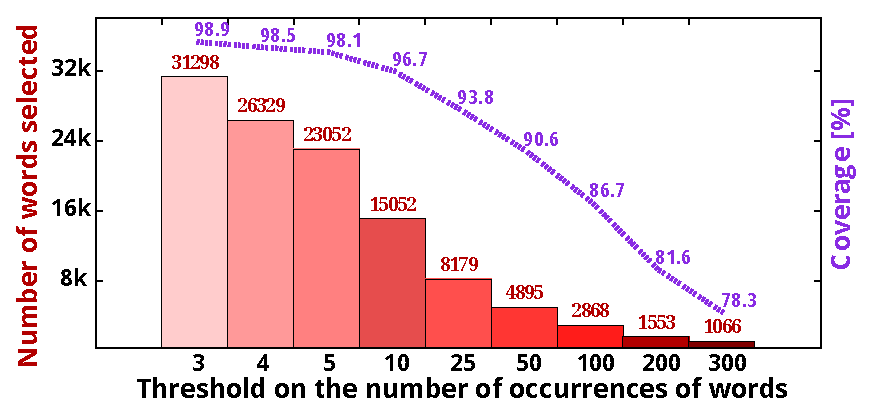
\includegraphics[scale=1.45]{Image/results/couverture_ws_minocc}
			\end{center}

		\item {\color{OrangeRed} How many syllables} are modeled inside the hybrid LM?
			\vskip1.3ex
			\begin{center}
			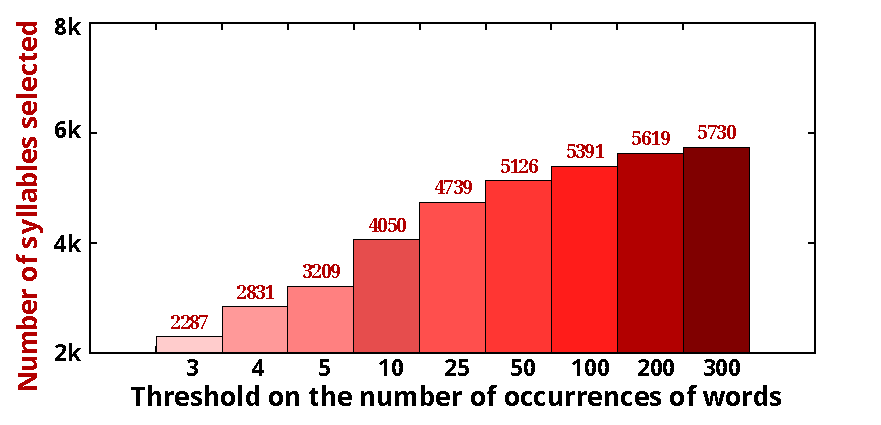
\includegraphics[scale=1.45]{Image/results/couverture_ws_s_minocc}
			\end{center}
		\end{itemize}

	\end{block}


}

\end{minipage}
\end{beamercolorbox}
\end{column}

% ---------------------------------------------------------%
% Set up a column
% ---------------------------------------------------------%
\begin{column}{.36\textwidth}
\begin{beamercolorbox}[rounded=true,center,wd=\textwidth]{postercolumn}
\begin{minipage}[T]{.98\textwidth}

\parbox[t][\columnheight]{\textwidth}
{
	\vskip.1ex

	\begin{block}{Retrieving the message carried out by the speech signal}
		\vskip-1.1ex
		\begin{columns}
		\begin{column}{.50\textwidth}
			\begin{center}
			{\color{OrangeRed} How many words} are  \\
			generated by the decoder?
			\vskip1.5ex

			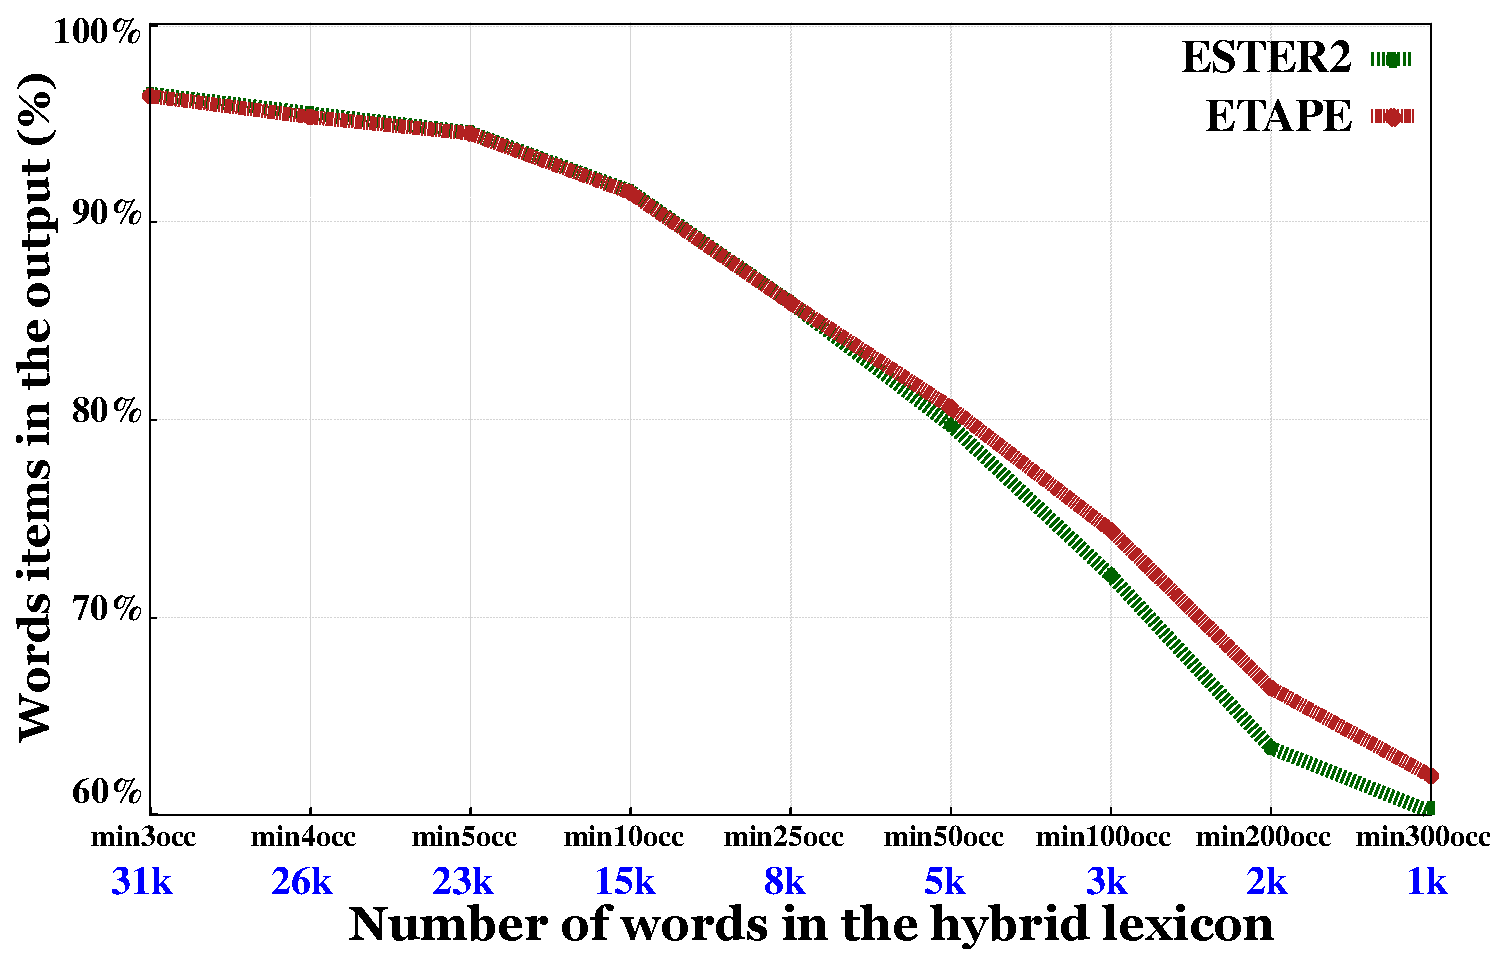
\includegraphics[scale=0.79]{Image/results/wordsInWS}
			\end{center}
		\end{column}
		\begin{column}{.50\textwidth}
			\begin{center}
			Among these words, how many  \\
			of them were {\color{OrangeRed} correctly recognized} ?
			\vskip1.5ex

			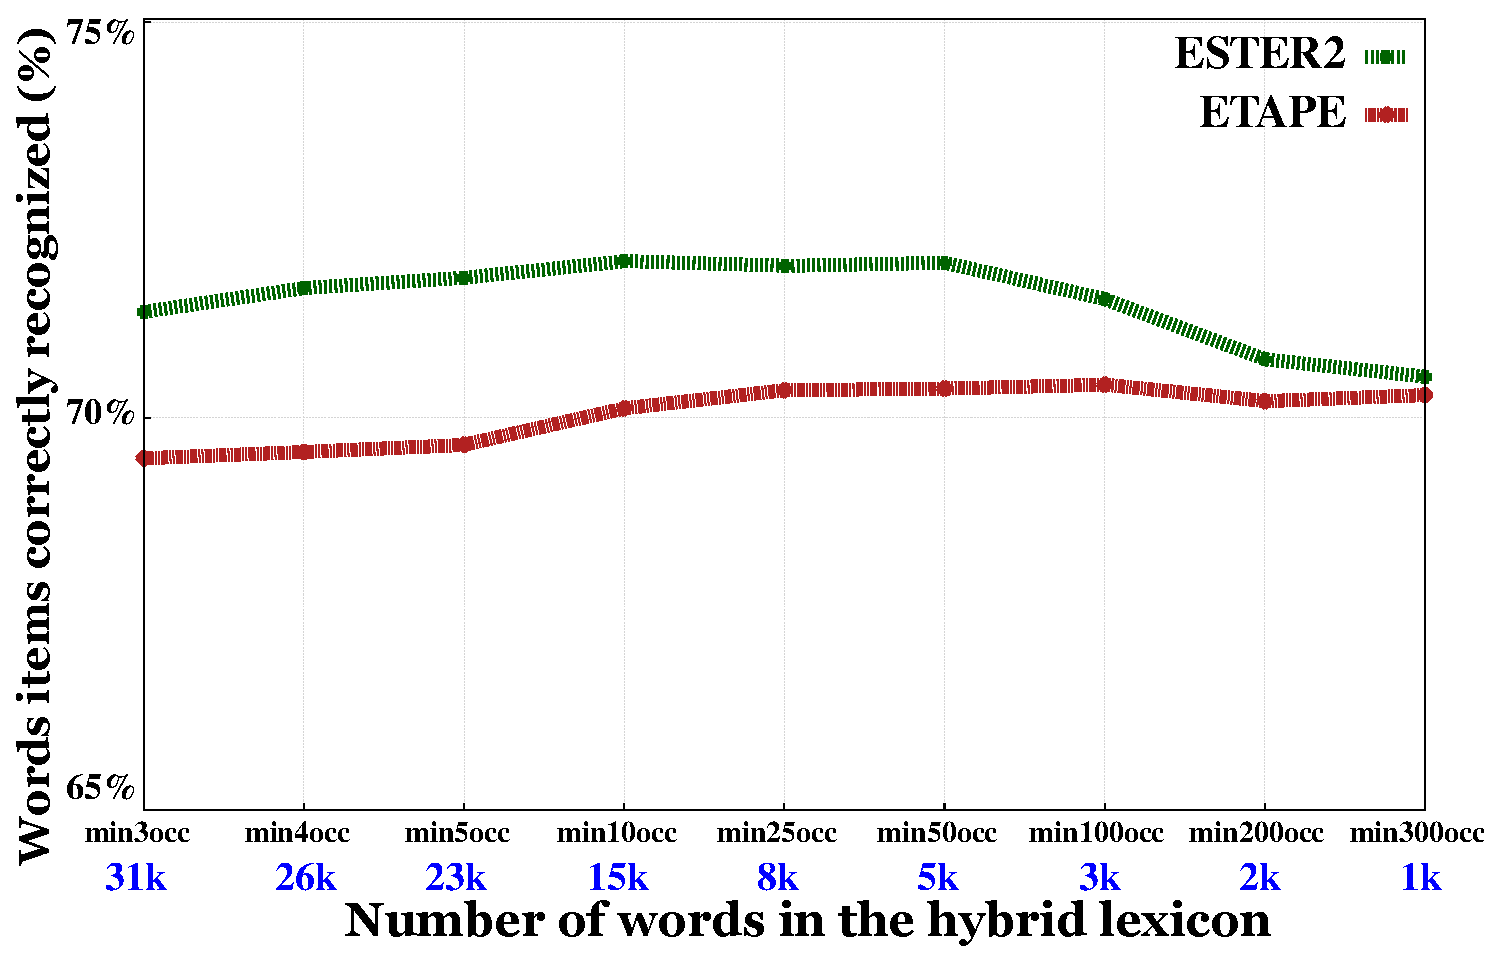
\includegraphics[scale=0.79]{Image/results/correctWordsInWS}
			\end{center}
		\end{column}
		\end{columns}

		\vskip3ex
		{\color{blendedblue} \hrule }
		\vskip3ex

		\begin{center}
		\vskip0.5ex
		Can the confidence measures identify correct items?
		\end{center}
		\begin{columns}
		\begin{column}{.50\textwidth}
			\begin{center}
			\vskip-1.5ex
			{\color{OrangeRed} correctly recognized words?}
			\vskip1ex
			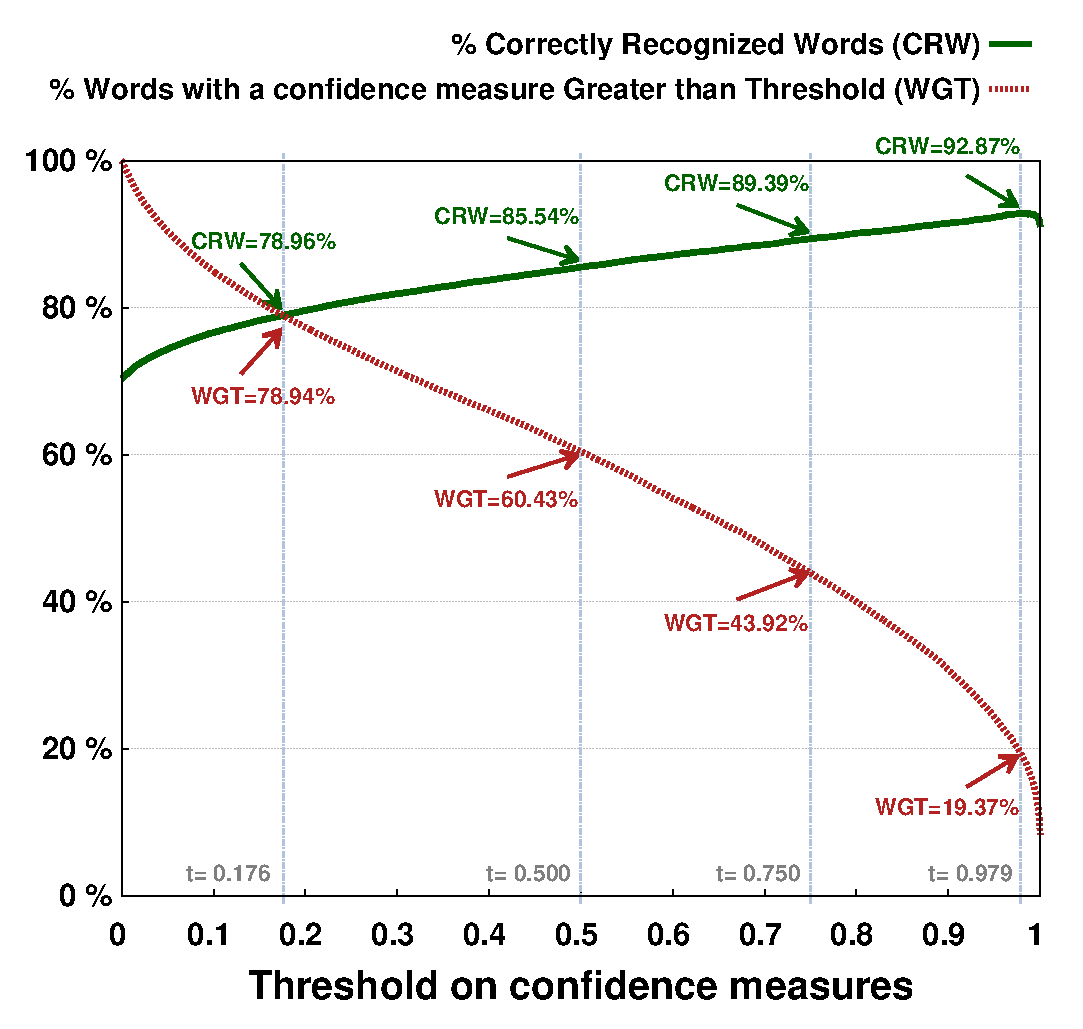
\includegraphics[scale=1.13]{Image/results/ETAPE_combined_min50occ_words}
			\end{center}
		\end{column}
		\begin{column}{.50\textwidth}
			\begin{center}
			\vskip-1.5ex
			{\color{OrangeRed} correctly recognized syllables?}
			\vskip1ex
			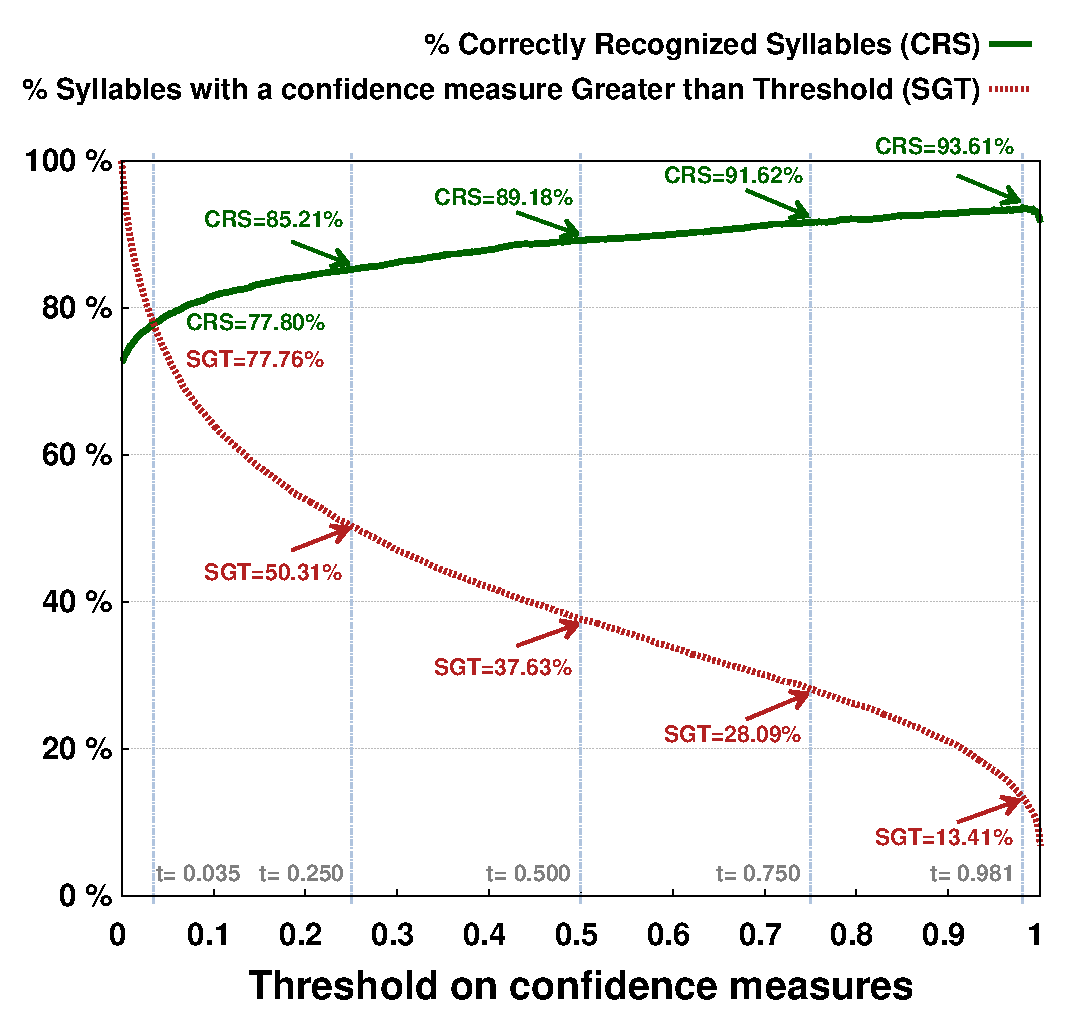
\includegraphics[scale=1.13]{Image/results/ETAPE_combined_min50occ_syllables}
			\end{center}
		\end{column}
		\end{columns}
		\vskip1ex
		\textbf{\footnotesize Evaluation on ETAPE corpus, hybrid lexicon with 5k word entries}
	\end{block}

	\vskip0.65ex
	\begin{block}{Conclusions}
		\vskip-.9ex
		\begin{itemize}
			\item the hybrid language model is a good compromise
			\item among the recognized words which have a confidence measure greater than 0.5, 85\% are correctly recognized
			\item evaluations have also shown that the contribution of confidence measures on syllables is relevant only if there is a fairly significant amount of syllables in the language model
		\end{itemize}
	\end{block}

	\vskip0.65ex
	\begin{block}{Future work}
		\vskip-.9ex
		\begin{itemize}
			\item investigate further confidence measures on the syllables units
			\item towards detection of error zones instead of item-based decision
		\end{itemize}
	\end{block}
}


\end{minipage}
\end{beamercolorbox}
\end{column}
\end{columns}
\end{frame}
\end{document}

